\label{chap:refresh}
% List down refresh strategies
In this chapter, we discuss some of the refresh strategies we investigated.
Along with the description of the strategies, we also describe the motivation
which led us to designing them, and their potential impact on the behaviour of
the CAL algorithm, in terms of effectiveness and efficiency. When applicable, we
also report results of supporting experiments which can help gain more insight
into some refresh strategies.

\section{Basic Concepts}
Before discussing the refresh strategies, it is useful to define few basic
concepts.
\subsection*{Effectiveness}
Effectiveness is the measure of utility the CAL system provides to its users. A
more effective system would let users find more relevant documents with lesser
review effort.  Chapter~\ref{chap:dataset} defines in detail how we measure the
effectiveness.

\subsection*{Efficiency}
We use the term efficiency to indicate the computation costs of the CAL system.
While memory costs should also be a factor when evaluating efficiency, we are
mostly concerned with the CPU costs and running times in this thesis.

\subsection*{Responsiveness}
Responsiveness of a CAL system becomes important in the context of live and
interactive systems. In a real world application, system delays in delivering
documents for review can be detrimental to user experience and waste valuable
assessor time. A responsive system should minimize all such delays without
harming its effectiveness. One way to improve responsiveness is through
efficiency.  Other ways include utilizing the idle time when the reviewer is
reading the document.

\subsection*{Full Refresh}
We use the term \textit{full refresh} to denote a refresh in which all
available judgments are used in training and relevance likelihood scores for all
the documents are calculated.

A full refresh runs in $O(t + n\log n)$ time where $n$ is the number of
documents in the corpus and $t$ is the number of training iterations. The number
of iterations $t$ required for convergence depends on the size of the training data
(or number of judgments). We set $t$ to a high constant value ($100000$) for our
dataset. Although the length of documents (specifically, the number of
non-zero features in a document feature vector) affect the running time of training
and scoring, we treat it as a constant to simplify our analysis. Scoring all the
documents takes $O(n)$ time and sorting them takes $O(n \log n)$ time. In most
cases, only top $k$ documents (where $k<<n$) are needed. In such cases, complete
sorting is not required and the refresh can be performed in $O(t + n \log k)$
time.

\section{BMI}

In the original BMI AutoTAR, full refreshes are performed after receiving a
batch of judgments. The size of this batch increases exponentially with number
of refreshes. The batch size is initially set to $k=1$ and after every refresh,
is updated using
\begin{equation*}
k \leftarrow k + \lfloor\frac{k + 9}{10}\rfloor
\end{equation*}

The smaller batch size during the beginning of a task results in frequent
refreshes and thus allows the classifier to frequently update its understanding
of relevance. This strategy scales well with the number of judgments ($E$) made
during the CAL process since only $O(\log E)$ number of refreshes are done.
According to the authors of BMI, the motivation behind this strategy was to
``\textit{reap the benefits of early precision, while avoiding downside risk and
    excessive running time, by using exponentially increasing batch
size}''~\cite{cormack2015autonomy}.

\section{Static Batch}

The simplest refresh strategy. In \textit{static batch refresh strategy}, full
refreshes are performed after a fixed number of judgments are received. When
batch size is fixed to $1$, a full refresh happens after every judgment. The
only parameter in this strategy is the judgment batch size.

This strategy incurs a high computation cost and introduces scalability issues
since it requires $O(E)$ number of refreshes and each refresh takes $\Omega(n)$
time, where $E$ is the number of documents judged during the CAL process and
$n$ is the number of documents in the dataset.

\subsection{Responsiveness}
\label{sec:async}
If a judgment triggers a refresh, the system waits for the refresh to complete
before returning a fresh set of documents for the user to judge.
For very small batch sizes (such as $1$) and large values of $n$, full refreshes
will be frequent and expensive. Pauses as small as half a second after every few
judgments can disrupt the user experience.

One way to address this problem is to perform asynchronous refreshes and
immediately show the users documents from the old review
queue~\cite{sigirdemo}. During a refresh, we fill the review queue
with few extra top documents in addition to the batch size. Whenever a judgment
triggers a refresh, we delegate the refreshing to a background process and
continue serving the user the aforementioned extra documents from the review
queue. Meanwhile, when the refresh in the background is finished, the review
queue is replaced with a newer version. This modification delays the effect of
user feedback on the review queue by $\lceil\frac{t_r}{t_u}\rceil$ documents,
where $t_r$ is the time it takes to complete a refresh, and $t_u$ is the time a
user takes to review one document.

UWaterlooMDS in TREC 2017 Core Track~\cite{zhang2017uwaterloomds} used CAL to
power their manual review tool.  They used asynchronous static batch strategy
with batch size of 1. The tool presented summaries in addition to the full
document to the reviewers.  The authors and a group of graduate students used
the review tool to judge numerous documents in the New York Times collection
across 250 topics. The average and median time spent on a judgment were 13 and
4.1 seconds respectively. We simulated their judgments using our system and the
average refresh time was 1.71 seconds. Thus, for both average and median user
judgment times, the effect of user feedback is delayed by 1 document! \red{Fix
the average refresh time. It will be lower since it is currently based on
scoring paragraphs rather than documents}.

\begin{figure}[h]
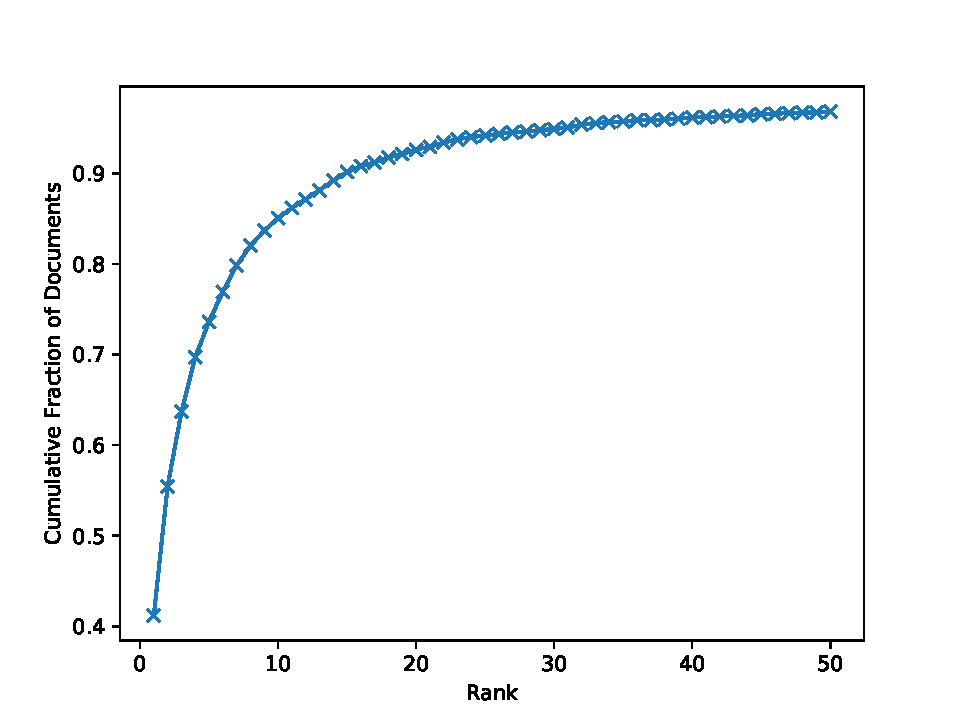
\includegraphics[width=\textwidth]{plots/top_doc_avg_rank.pdf}
\caption{Avg. fraction of currently second-ranked documents vs the rank below
which they were placed after the background refresh}
\label{plot:async}
\end{figure}

When the effect of user feedback is delayed by 1 document, the assessor ends up
judging the top two documents from the current review queue before the new
review queue is ready. To estimate the quality of the second
document showed to the user, we obtained the rank of that second document
in the next review queue (the review queue populated by the background refresh).
The setup for this experiment is described in Appendix~\ref{AppendixB}. We found that
$41.2\%$ of these documents were top ranked after the background refresh.
Moreover, $85\%$ and $96.8\%$ of these documents were ranked top 10 and top 50
respectively, after the background refresh. Figure~\ref{plot:async} plots the
percentage of documents which were within some given top ranks after the
background refresh.



If the CAL system can perform two refreshes while the user is reading a
document (i.e. $2t_r \le t_u$), we can achieve a responsive system without any
delay in processing of judgments. If the user is reading a document and his
judgment will trigger a refresh, a background process can just perform two refreshes;
one assuming the upcoming judgment will be relevant, and another assuming it
will be non-relevant.  The two possible future review queues are therefore ready
while the user is reading the document and the correct one can be immediately
served once the user judgment is received. For the numbers provided in the
previous paragraph, the constraint $2t_r \le t_u$ hold true.

\section{Partial Refresh}
\label{sec:partial}

In this strategy, a full refresh is performed after every fixed number of
judgments, similar to the \textit{static batch strategy}. At the end of each
full refresh, a small set of documents with the highest relevance likelihood
scores are stored in a \textit{partial refresh set}. After every judgment, a
\textit{partial refresh} is performed. During a partial refresh, all available
judgments are used in training but relevance likelihood scores are only
calculated for the documents in the partial refresh set. A single partial
refresh runs in $O(s\log{s})$ average time, where $s$ is the size of the
\textit{partial refresh set}. There logarithmic factor in running time
is a result of the partial set stored as a binary search tree and after every
judgment, it takes $O(\log(s))$ time to remove a document from that set. Since
the scores for the document in this set are recomputed after every
judgment, only the document with maximum score is returned to the user.

Partial refresh strategy has two parameters:
\begin{itemize}
    \item $k$: number of judgments between two full refreshes
    \item $s$: size of the partial refresh set (should not be less than $k$)
\end{itemize}

\begin{figure}[]
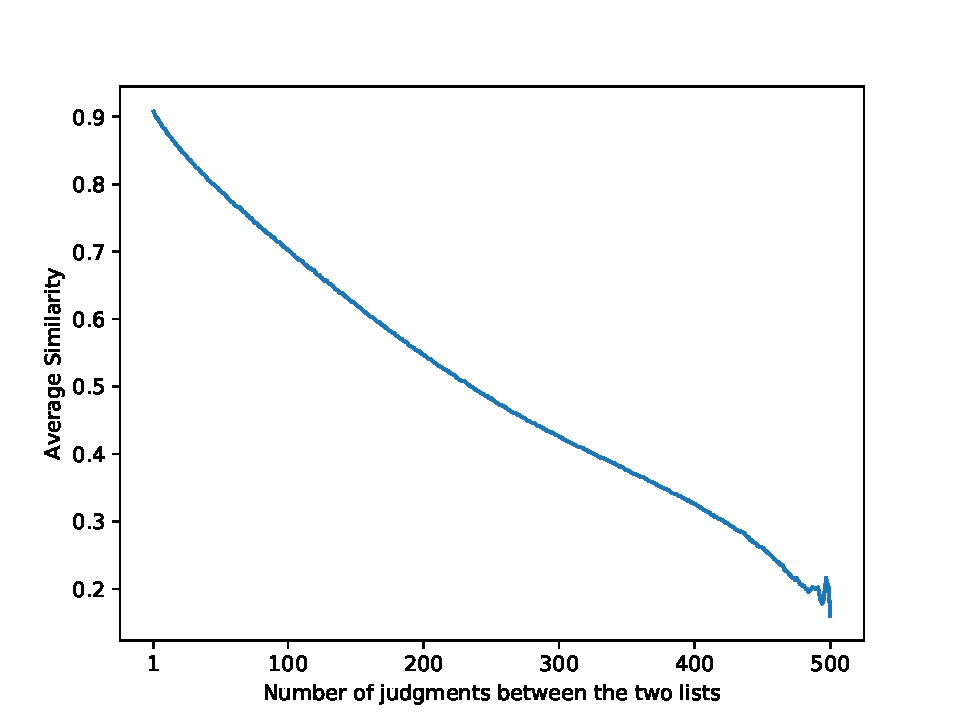
\includegraphics[width=\textwidth]{plots/ranklist_similarity.pdf}
\caption{Average similarity between two ranked lists (truncated at 1000)
separated by various number of judgments. Similarity between two lists is
computed as the fraction of common documents between them.}
\label{plot:partial}
\end{figure}

Our motivation behind designing this strategy was to efficiently replicate the
behaviour of \textit{static batch strategy} (batch size = $1$). We hypothesized
that the classifier's notion of relevance does not change dramatically between
two nearby judgments and we can safely avoid computing scores for low ranked
documents. To get some evidence, we constructed an experiment (the setup for
this experiment is explained in Appendix~\ref{AppendixB}). After each judgment, we stored
the list of top 1000 unjudged documents scored by the classifier. Since we
employed the static batch strategy with batch size of $1$, a refresh occurred
after every judgment. Similarity between two lists was computed as the fraction
of documents present in both lists.  Figure~\ref{plot:partial} reports the
average similarity of these document lists separated by various number of
judgments. $90.8\%$ of the top documents remain the same across consecutive
judgments (i.e., separated by 1 judgment). For the any two lists separated by
100 judgments, there were $70.3\%$ common documents in the top 1000.  The
results of the above experiment can also be qualitatively analysed to determine
the parameters for partial refresh strategy. For example, based on our results,
setting partial set size to 1000 and full refreshing every 100 judgments looks
like a reasonable starting point.

With some enhancements, this strategy can also help reduce the memory costs
when working with low physical memory or very large datasets (such as ClueWeb).
As mentioned in Section~\ref{sec:cal.design}, the documents are loaded in memory
to enable faster operations and improve the responsiveness of the system.
Partial refreshes are fast and performed on a small set of data which can be
stored in the memory. Full refresh can be performed in the background, and can
thus afford reads from the disk without sacrificing the user experience or
effectiveness of this strategy.

\section{Precision Based Refreshing}

The previous strategies we discussed use the elapsed number of judgments as
a criteria to determine when to refresh. Instead of number of judgments, we can
perform a full refresh when the ``output quality'' of the CAL system falls below
some threshold. The output quality of a CAL system is considered high if the
user judges more documents as relevant. There could be various ways to
concretely define ``output quality''.

In \textit{precision based refreshing}, we work with a very simple definition of
``output quality''. It is the fraction of relevant judgments in some fixed
number of latest judgments made by the reviewer. A full refresh is performed
whenever this fraction falls below some threshold. There are two parameters in
this strategy:
\begin{itemize}
    \item $m$: number of recent judgments to compute precision on
    \item $p$: the threshold below which a full refresh is triggered
\end{itemize}

Our aim is to find more meaningful factors which can help us better understand
the effectiveness of various refresh strategies, and as a result, help us design
better refresh strategies. For example, in certain cases, it is desirable to
save computation by not refreshing when the output quality is high and force
more frequent refreshes when the output quality is low. However, during later
stages of a task when the output quality is always low and the likelihood of
finding relevant documents is very low, \textit{precision based refreshing}
behaves similar to \textit{static batch refreshing} with batch size of $1$.

% This
% is undesirable as frequent refreshing at this stage of a task don't have any
% positive effect.\red{show data. how at later stages, training data and trained
% weights changes by very little with addition of one non-relevant document}.

\section{Prioritizing Recent Judgments}

\subsection{Recency Weighting Strategy}
\label{sec:recency}
This strategy modifies the training step (step 4 in Algorithm~\ref{alg.cal}) in
the CAL process by favoring documents which were recently judged. As described
in Section~\ref{sec:cal}, training is done over several iterations. In each
iteration of the original training, a relevant and a non-relevant document is
randomly sampled from the training set. The loss computed using them is used to
update the classifier weights. To incorporate recency weighting, we modified the
uniform random sampling such that the probability of selecting a document
increases if it was judged recently.

Given a list of documents $[D_1, D_2, ..., D_n]$ ordered by the time
they were judged, our modified random sampling will
select a document $D_x$ with probability $P(D_x)$ where

\begin{equation*}
P(D_x) = P(D_1) + \frac{P(D_1)(x-1)(w-1)}{N-1}
\end{equation*}

Therefore, $P(D_x)$ is a linear function such that the latest judged document
$D_n$ is $w$ times more likely to be selected than the oldest judged document
$D_1$. A full refresh (with modified training) is performed after every
judgment. The only parameter for this strategy is $w$.

Implementing the modified random sampling by computing the individual
probabilities of documents as shown in the above expression is inefficient. The
probabilities will have to be computed for all the documents in the training set
before every refresh. To achieve minimum overhead from the modified sampling, we
use a transformation on the uniform random number generator to achieve our
desired distribution. Appendix~\ref{AppendixA} covers the implementation of our
modified sampling in further detail.

\subsection{Number of Training Iterations}
Scoring can be made efficient by using strategies like \textit{partial
refreshing} or simply performing it over multiple processes. The choice of
training methods in the CAL algorithm makes it difficult to parallelize. There are
alternative training methods which are designed for efficiency and scalability,
but that is a direction for future work. A parameter in our training algorithm
which can be easily controlled and has a significant impact on performance is
the number of training iterations. Reducing the training iterations by some
factor significantly improves running time by sacrificing the effectiveness
of the system.

Our initial motivation behind \textit{recency weighting} was to improve the
default training
by prioritizing newer judgments. However, we found no difference in
effectiveness of CAL between the original and modified training. We
shifted our efforts towards using recency weighting to improve the effectiveness
of training with low number of iterations.


\begin{table}[]
\centering
\caption{List of the refresh strategies and their parameters.}
\label{table.strategies}
\begin{tabular}{|c|c|}
\hline
\textbf{Strategy} & \textbf{Parameters} \\ \hline \hline
\texttt{bmi} & None \\ \hline
\texttt{static} & $k$ = \textit{no. of judgments between full refreshes} \\ \hline
\texttt{partial} & \begin{tabular}[x]{@{}c@{}}
$k$ = \textit{no. of judgments between full refreshes} \\
$s$ = \textit{no. of documents in the partial refresh}\\
\textit{set}
\end{tabular} \\ \hline
\texttt{precision} & \begin{tabular}[x]{@{}c@{}}
$m$ = \textit{no. of recent judgments to}\\
\textit{compute precision on} \\
$p$ = \textit{full refresh is triggered if the precision of} \\ 
\textit{last $m$ documents fall below this value}
\end{tabular} \\ \hline
\texttt{recency} & \begin{tabular}[x]{@{}c@{}}
$w$ = \textit{factor by which the latest judged} \\
\textit{document is more likely to be sampled}\\
\textit{than the oldest judged document}
\end{tabular} \\ \hline
\texttt{*} & \begin{tabular}[x]{@{}c@{}}
$it$ = \textit{no. of training iterations} \\
\textit{(global parameter, $100000$ unless specified)}
\end{tabular} \\ \hline
\end{tabular}
\end{table}
